\documentclass[answers]{exam}

% ------------------------------------------------------------------------------ %
% -----------------------      Base for every .tex file   ---------------------- %
% ------------------------------------------------------------------------------ %

\usepackage[dvipsnames]{xcolor}
\usepackage{mathtools}
\usepackage{amssymb}
\usepackage{amsthm}
\usepackage{amsmath}
\usepackage{framed}
\usepackage{wasysym}
\usepackage{geometry}
\usepackage{cancel}
\usepackage{blindtext}
\usepackage{pgfplots}
\usepackage{graphicx}
\usepackage{lastpage}
\usepackage[most]{tcolorbox} 
\usepackage{multicol}
\usepackage{soul}
\usepackage{listings}
\usepackage{algorithm}
\usepackage{algorithmic}
\usepackage{booktabs}
\usepackage{tikz}
\usepackage{pifont}

% Libraries
\usetikzlibrary{shapes,shapes.geometric, positioning, arrows}

\geometry{%
	left=15mm,
	right=15mm,
	top=25mm,
	bottom=25mm,
	bindingoffset=0mm,
	headheight=30pt,% output from geometry tells you what this needs to be set to as a minimum
}

% Header and Footer
\pagestyle{headandfoot}
\firstpageheadrule
\runningheadrule
\firstpageheader{Convex Optimization}{\today}{Jonathan Schnell}
\runningheader{Convex Optimization}{}{Jonathan Schnell}
\firstpagefooter{}{Page \thepage\ of \numpages}{}
\runningfooter{}{Page \thepage\ of \numpages}{}

% Commands
\newcommand{\imp}[1]{\ul{\textbf{#1}}}
\newcommand{\dproduct}[1]{\left\langle #1 \right\rangle}
\newcommand{\norm}[1]{\left\lVert #1 \right\rVert}
\renewcommand{\vector}[1]{\begin{pmatrix} #1 \end{pmatrix}}
\newcommand{\abs}[1]{\left| #1 \right|}
\newcommand{\floor}[1]{\lfloor #1 \rfloor}
\newcommand{\ceil}[1]{\lceil #1 \rceil}
\newcommand{\fracpart}[2]{\frac{\partial #1}{\partial #2}}
\newcommand{\set}[2]{\left\{#1 \ \middle|\ #2\right\}}
\renewcommand{\hat}[1]{\widehat{#1}}

\newcommand{\Ker}{\operatorname{Ker}}
\renewcommand{\Im}{\operatorname{Im}}
\renewcommand{\Re}{\operatorname{Re}}
\renewcommand{\dim}{\operatorname{dim}}
\renewcommand{\div}{\operatorname{div}}
\newcommand{\rot}{\operatorname{rot}}
\newcommand{\grad}{\operatorname{grad}}
\newcommand{\vol}{\operatorname{vol}}
\newcommand{\supp}{\operatorname{supp}}
\renewcommand{\div}{\operatorname{div}}
\newcommand*{\vertbar}{\rule[-1ex]{0.5pt}{2.5ex}}
\newcommand*{\horzbar}{\rule[.5ex]{2.5ex}{0.5pt}}

\theoremstyle{definition}
\newtheorem*{definition}{Definition}
\newtheorem*{beispiel}{Beispiel}
\newtheorem*{remark}{Remark}

\theoremstyle{plain}
\newtheorem*{proposition}{Proposition}
\newtheorem*{satz}{Satz}
\newtheorem*{korollar}{Korollar}
\newtheorem*{lemma}{Lemma}
\newtheorem*{theorem}{Theorem}


% Quote
\newtcolorbox{zitat}[1]{%
	colback=lightGray,
	grow to right by=-10mm,
	grow to left by=-10mm, 
	boxrule=0pt,
	boxsep=0pt,
	breakable,
	enhanced jigsaw,
	borderline west={4pt}{0pt}{gray},
	#1
}

% Use colors in equations
\newcommand{\highlight}[2]{\colorbox{#1}{$#2$}}%
\definecolor{lightGray}{gray}{0.9} 

% To add shortcut of script Letters in Equations
\newcommand{\s}[1]{\mathcal{#1}}
\newcommand*\circled[1]{\tikz[baseline=(char.base)]{
            \node[shape=circle,draw,inner sep=2pt] (char) {#1};}}
\newcommand{\cmark}{\ding{51}}
\newcommand{\xmark}{\ding{55}}


\newenvironment{claim}[1]{
		\par\noindent
		\textbf{Claim.} #1
		\begin{tcolorbox}[blanker, top=3mm, bottom=3mm, left=3mm, borderline west={1pt}{0mm}{black}]
		\noindent\textit{Proof of Claim.} 
}{
	\hfill$\blacksquare$	
	\end{tcolorbox}\noindent
}

% To add shortcut of number's set Z
\newcommand*{\Z}{\mathbb{Z}}
\newcommand*{\N}{\mathbb{N}}
\newcommand*{\R}{\mathbb{R}}
\newcommand*{\Q}{\mathbb{Q}}
\newcommand*{\C}{\mathbb{C}}
\newcommand*{\F}{\mathbb{F}}
\newcommand*{\K}{\mathbb{K}}

% To add shortcut of empty set
\renewcommand*{\o}{\varnothing}
\pgfplotsset{compat=1.9}

\everymath{\displaystyle}

% Line-Height
\linespread{1.15}

\graphicspath{{Files/}}

% ------------------------------

\begin{document}

	$ $
	\begin{center}
		\huge \textbf{Exercise session notes - Week 5}  \\ \vspace*{3mm}
        \Large{Strong Duality + KKT points}
	\end{center}
	$ $\\

    \noindent Let's consider a general mathematical program
    \begin{align*}
        \min \quad f(x) & \\ 
        g_i(x) &\leq 0 \quad\forall i\\
        h_j(x) &= 0 \quad\forall j
    \end{align*}
    Last week we constructed the Lagrange Dual Program as follows 
    \begin{align*}
        \min \quad \hat{L}(\lambda, \nu)& \\ 
        \lambda \geq 0
    \end{align*}
    where the objective function is the Lagrange dual function, defined as 
    $$ \hat{L}(\lambda, \nu) = \inf_x\Big\{ f(x) + \sum \lambda_i g_i(x) + \sum \nu_j h_j(x)\Big\} $$
    We now list some properties about duality. \\
    \paragraph{Proposition.} (Weak Duality) For any program we have 
    $$\max \hat{L}(\lambda, \nu) \leq \min f(x)$$
    \paragraph{Definition.} (Strong Duality) We say strong duality holds if the duality gap is $0$, i.e.  
    $$\max \hat{L}(\lambda, \nu) = \min f(x)$$
    \paragraph{Proposition.} (Complementary Slackness) If strong duality holds, then for any optimal primal-dual solution $(x^*, \lambda^*, \nu^*)$ we have 
    $$\lambda_i^* \cdot g_i(x^*) = 0\quad\quad \forall i $$
    This means that for each $i$, either the $i$th primal constraint is tight ($g_i(x) = 0$) or the $i$th dual constraint is tight ($\lambda_i = 0$), or both of them are tight. 
    \paragraph{Definition.} (KKT-conditions) A point $(x,\lambda, \nu)$ is a KKT-point if:
    \begin{alignat*}{3}
        \circled{1}\quad &\text{Primal feasible}\quad &&:\quad g_i(x)\leq 0;\ h_j(x) = 0 \\ 
        \circled{2}\quad &\text{Dual feasible}\quad &&: \quad \lambda_i\geq 0 \\
        \circled{3}\quad &\text{Comp. slackness}\quad &&: \quad \lambda_i\cdot g_i(x) = 0 \\ 
        \circled{4}\quad &\text{Gradient vanishes}\quad &&:\quad \nabla_x L(x,\lambda, \nu) = 0
    \end{alignat*}

    \paragraph{Proposition.} For \underline{any} mathematical program: 
    $$ \text{Strong Duality holds} + \text{$(x,\lambda,\nu)$ is optimal} \implies \text{$(x, \lambda, \nu)$ is KKT point} $$
    \paragraph{Proposition.} For \underline{convex} mathematical programs: 
    $$ \text{Strong Duality holds} + \text{$(x,\lambda,\nu)$ is optimal} \iff \text{$(x, \lambda, \nu)$ is KKT point} $$

    Now we show an example of a convex mathematical program for which Strong duality does not hold. 

    \paragraph{Example.} Consider the following program (P)
    \begin{align*}
        \min \quad e^{-x} & \\ 
        \frac{x^2}{y} &\leq 0
    \end{align*}
    where we set the domain as $\s{D} = \set{(x,y)}{y > 0}$. 
    % The feasibility set is the following
    % \begin{center}
    %     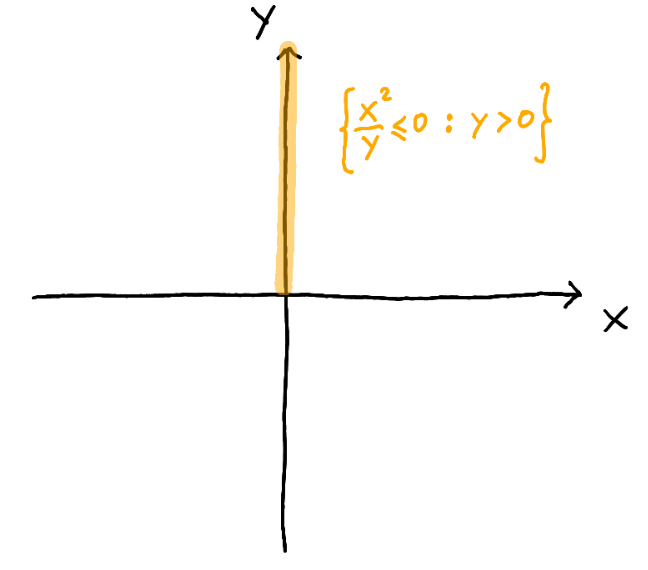
\includegraphics[width=0.25\textwidth]{FeasibleSet.png}
    % \end{center}
    Note that in this domain, the program is a convex program (Exercise). Moreover the optimal value is $\highlight{lightGray}{f^* = 1}$. We now compute the dual problem: Let $\lambda \geq 0$, then
    \begin{align*}
        &L(x,y,\lambda) = e^{-x} + \lambda \frac{x^2}{y} \\
        \implies & \hat{L}(\lambda) = \inf_{x,y} \Big\{e^{-x} + \lambda \frac{x^2}{y}\Big\}
    \end{align*}
    Since $y$ is positive, we have $L(x,y,\lambda) \geq 0$. Moreover if we let $x = n$, $y = n^3$ for $n\in \N$ and tend $n\to \infty$ we obtain 
    $$ L(n, n^3, \lambda) = e^{-n} + \lambda\frac{1}{n} \to 0 $$
    In particular we have $\hat{L}(\lambda) = 0$. With this, we can write the dual program (D) of (P) by 
    \begin{align*}
        \max \quad \hat{L}(\lambda) &= 0 \\ 
        \lambda &\geq 0
    \end{align*}
    with optimal value $\highlight{lightGray}{\hat{L}^* = 0}$. For this pair of programs we have a duality gap of $1$, so strong duality does not hold. By the previous proposition there exists no KKT point, so let's see what goes wrong. Consider a point $(x, y, \lambda)$ in the domain of the primal/dual programs and assume it is a KKT-point.
    \begin{itemize}
        \item[\circled{1}] We have $\tfrac{x^2}{y} = 0$ so $x = 0$. $\qquad \text{\cmark}$
        \item[\circled{2}] We have $\lambda \geq 0$. $\qquad \text{\cmark}$
        \item[\circled{3}] We have $\lambda\tfrac{x^2}{y} = \lambda\tfrac{0}{y} = 0$. $\qquad \text{\cmark}$
        \item[\circled{4}] We have $\nabla_{x,y} L = 0$ so
        $$ \frac{\partial}{\partial y} L = 0 - \lambda \frac{x^2}{y^2} = 0 \quad\text{\cmark}  $$
        and 
        $$ \frac{\partial}{\partial x} L = -e^{-x} + 2\lambda \frac{x}{y} = -e^{0} = -1 \neq 0\quad \text{\xmark}  $$
    \end{itemize}
    Therefore there are no KKT-points for this problem.

\end{document}